\documentclass[letterpaper,12pt]{article} % Font and paper size
\usepackage[utf8]{inputenc}
\usepackage[spanish]{babel}
\usepackage{graphics,geometry,tikz,circuitikz,siunitx,enumitem,amsmath}
\usepackage{wrapfig}
\usetikzlibrary{babel}
\decimalpoint

\geometry{letterpaper,left=1.5cm,right=1.5cm,top=2.0cm,bottom=2.0cm}

%\title{Analisis de circuitos RLC}
%\author{Alumno\\
%  \small Universidad \\
%  \small email\\
%  \small ubicación
%  \date{}}
%  
  \begin{document}
%\maketitle
% Encabezado -----------------------------------------------------------------
\noindent
\begin{minipage}{0.7\textwidth}
	\textbf{Universidad de Costa Rica - Sede de Guanacaste} \\
	\textbf{IE-0209 Circuitos Lineales I} \\
	\textbf{Primer Semestre del 2022} \\
	\textbf{Tarea \#6}
\end{minipage}
\noindent
\begin{minipage}{0.3\textwidth}
	\centering
	
\includegraphics[scale=0.65]{LogoEIE-SG.png}
\end{minipage}
\vspace{0.4cm}
\hrule
\vspace{0.4cm}
\section*{Descripción de elementos.}

Antes de analizar un circuito RLC empezaremos por describir cada uno de los elementos involucrados, es decir resistores (o resistencias), capacitores (o condensadores) e inductores (o bobinas). \\ \\

\subsection*{Resistor o resistencia}
Este componente será un material omhnico, es decir, que cumple con la ley de Ohm, esto implica que al aplicar que la diferencia de potencia $V_R$ requerida para que una corriente $I$ atraviese el resistor es igual al producto de dicha corriente y la resistencia $R$ del elemento. esto se puede expresar más formalmente como \eqref{lohm}.\\ 

\begin{equation} 
V_R=RI
\label{lohm}
\end{equation}

En un circuito, las resistencias se representan graficamente en diagramas de  circuitos mediante el simbolo mostrado en la figura \ref{fig:ressym}.\\
\begin{figure}[h]
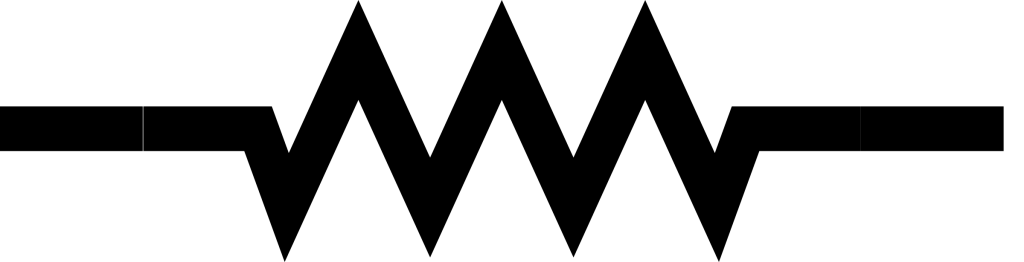
\includegraphics[scale=0.115]{res.png}
\centering
\caption{simbolo internacional del resistor}
\label{fig:ressym}
\end{figure}

\subsection*{Capacitor}

El capacitor es un dispositivo que almacena carga eléctrica cuando se aplica una diferencia de potencial $V_C$ entre sus extremos, la carga almacenada $q$ es proporcional al la diferencia de potencial aplicada, así como tambien al valor de la capacitancia $C$, la que podría definirse como la capacidad de almacenamiento de carga por unidad de potencial aplicada. Esto se expresa formalmente por medio de \eqref{qcap}.

\begin{equation}
q=V_CC
\label{qcap}
\end{equation}\\

Vale la pena resaltar que debido a que la intensidad de corriente que atraviesa un capacitor es equivalente a la derivada temporal de la carga almacenada, tambien podemos escribir \eqref{icap}.

\begin{equation}
I=\frac{dq}{dt}=C\frac{dV_C}{dt}
\label{icap}
\end{equation}

El simbolo utilizado para representar gráficamente estos dispositivos en un circuito es \ref{fig:capsym}.

\begin{figure}[h]
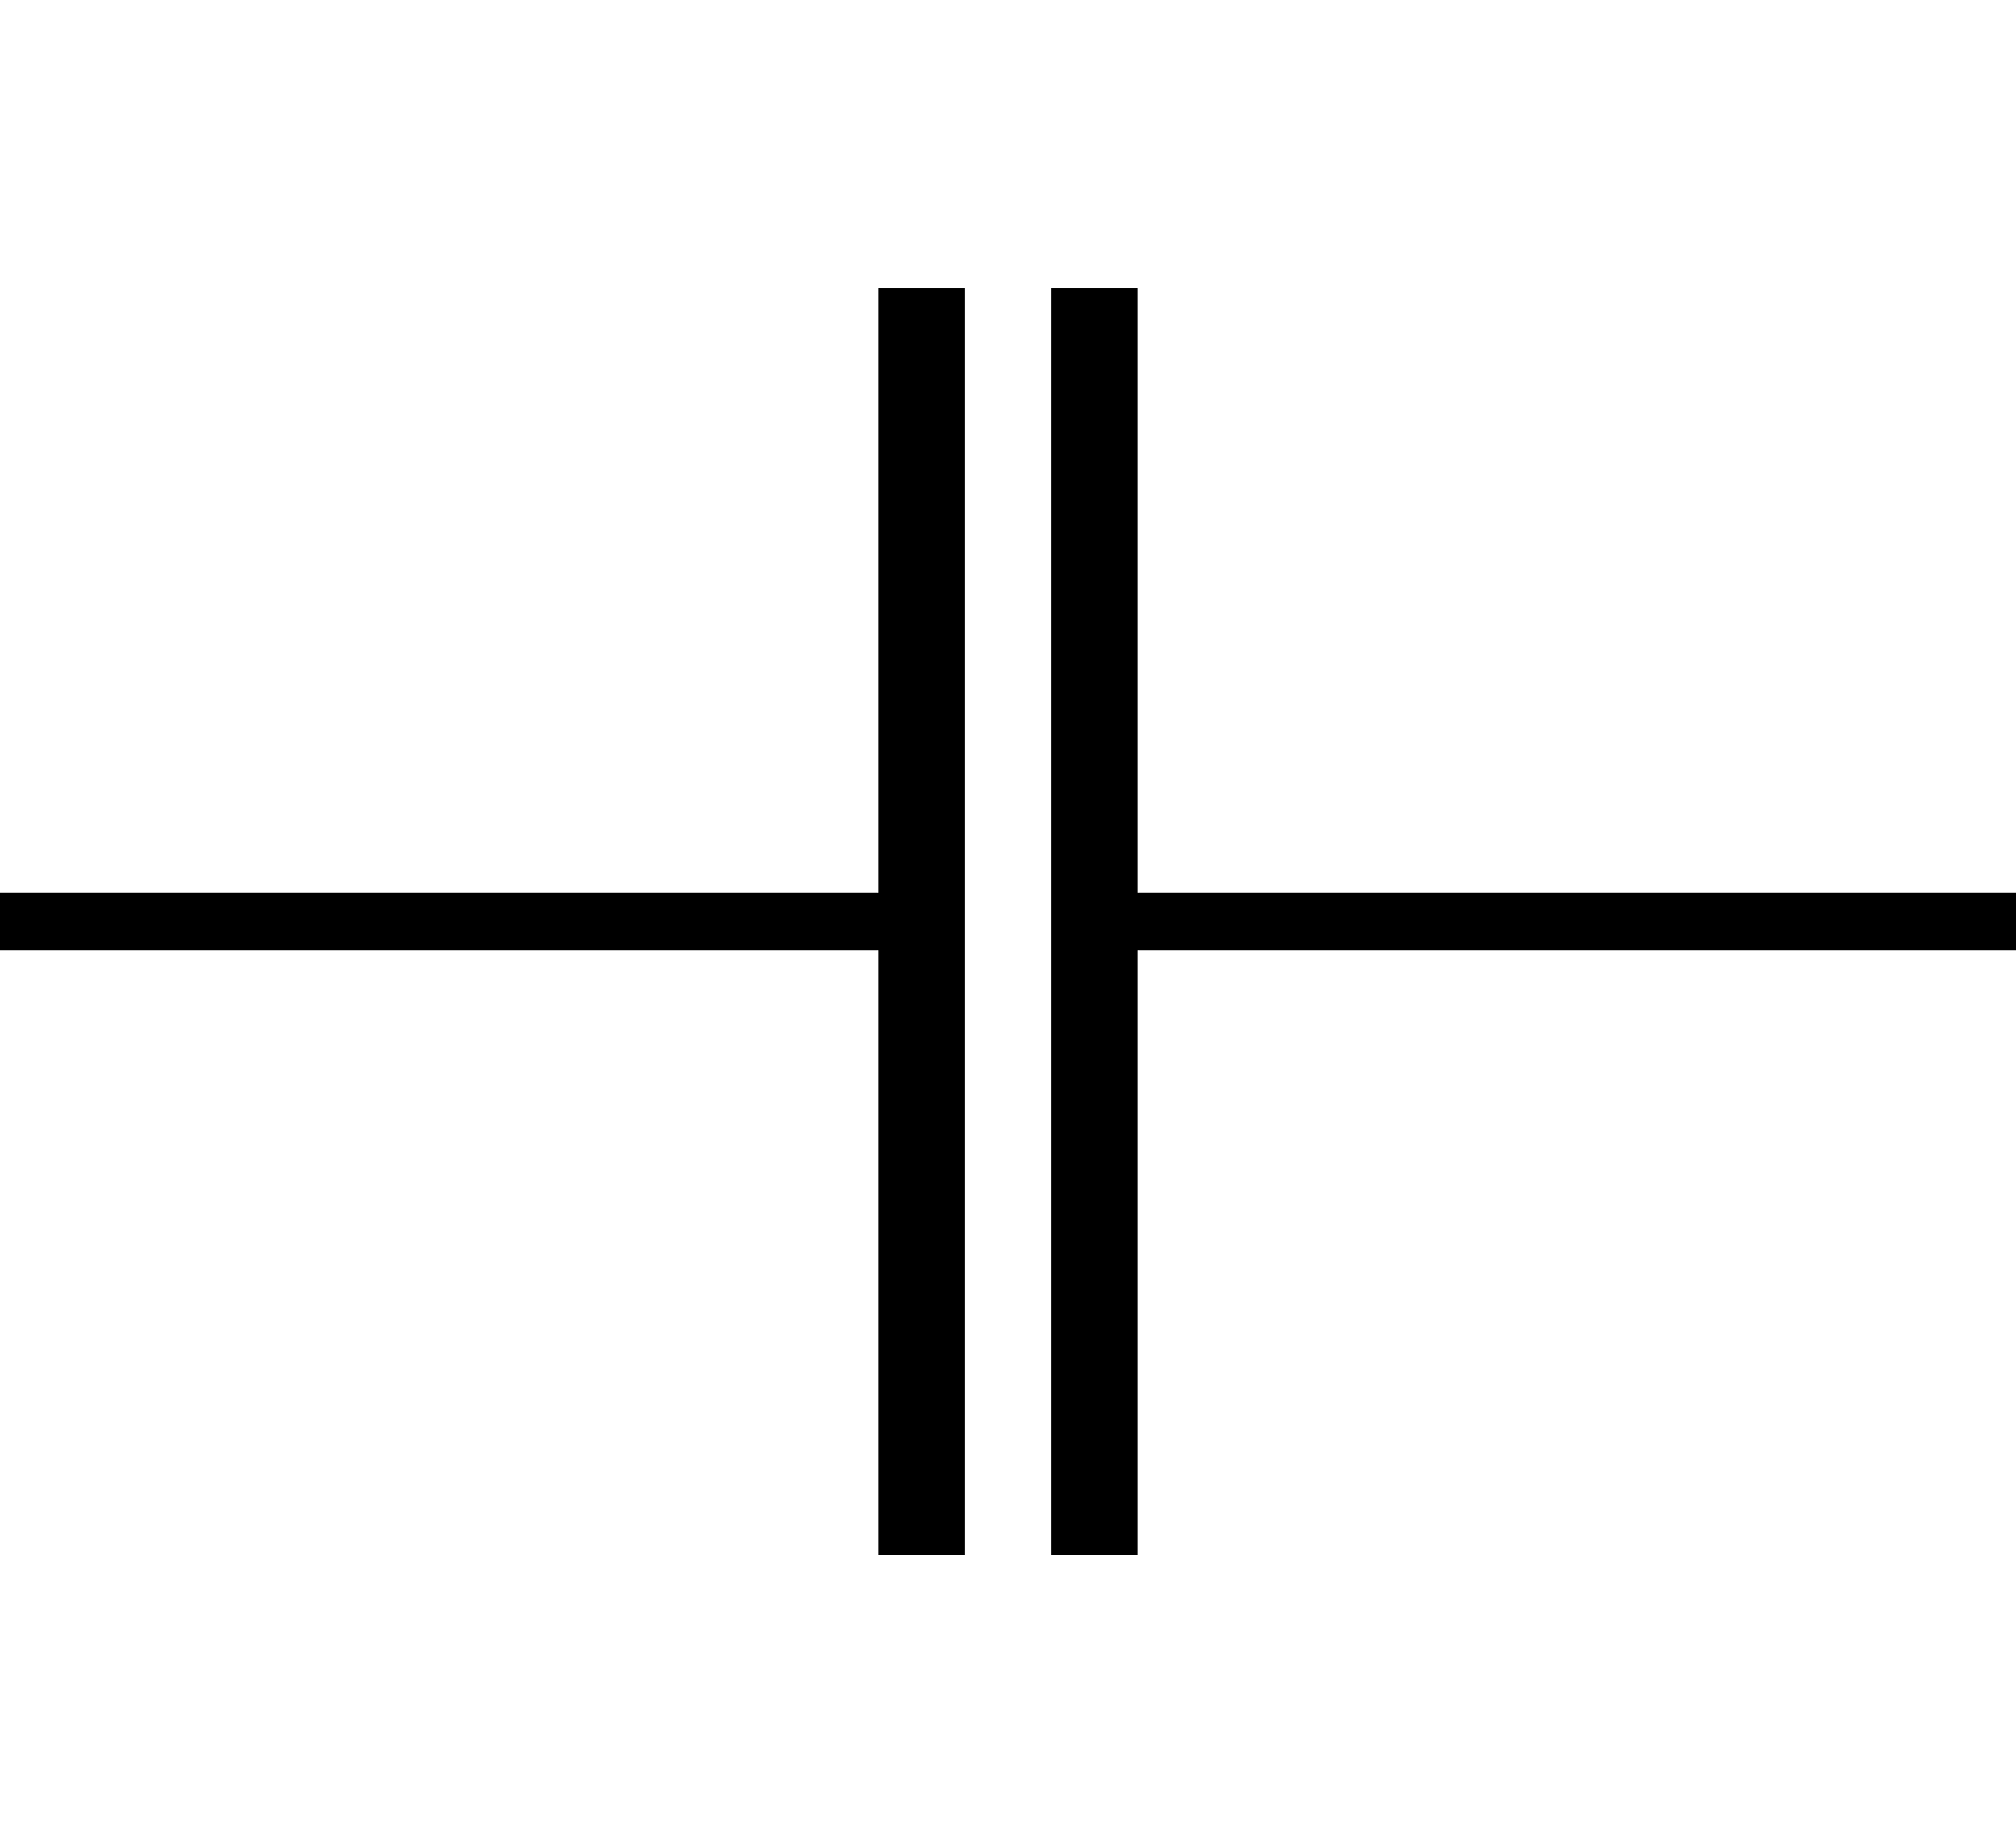
\includegraphics[scale=0.04]{capsym.png}
\centering
\caption{simbolo internacional del capacitor}
\label{fig:capsym}
\end{figure}

\subsubsection*{Reactancia}
El capacitor es un elemento reactivo, su reactancia puede expresarse como \eqref{xcap}. Donde $\omega$ es la velocidad angular de asociada a la corriente que atraviesa el capacitor.
\begin{equation}
X_C=-\frac{1}{\omega C}
\label{xcap}
\end{equation}

\subsection*{Inductor}

El inductor es, a rasgos generales, una bobina. Cuando una corriente electrica atraviesa el capacitor se genera un campo magnético que autoinduce al mismo dispositivo, en consecuencia, el capacitor es una elmento que opone resistencia al cambio en la intensidad de corriente. Matemáticamente podemos expresalor como \eqref{vind}.

\begin{equation}
V_L=L\frac{dI}{dt}
\label{vind}
\end{equation}

El inductor se representa gráficamente mediante un símbolo que asemeja un resorte o varias espiras, algunos de estos simbolos usuales son \ref{fig:indsym}.

\begin{figure}[h]
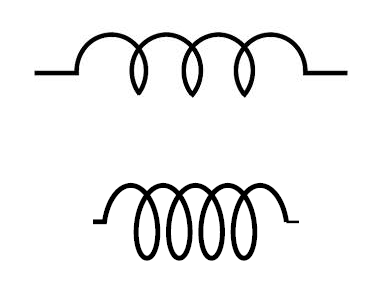
\includegraphics[scale=0.5]{indsym.png}
\centering
\caption{simbolos usuales para el inductor.}
\label{fig:indsym}
\end{figure}

\subsubsection*{Reactancia}
Los inducores, en principio, no ponen resistencia, pero así como los capacitores, los inductores tambien son elementos reactivos. La reactancia inductiva es decrita por \ref{xind}.
\begin{equation}
X_C=\omega L
\label{xind}
\end{equation}

\section*{Circuito RLC en serie}

\begin{wrapfigure}{r}{0.24\textwidth}
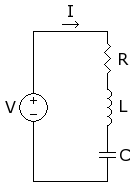
\includegraphics[scale=0.8]{rlcserie.png}
\centering
\caption{Circuito RLC en serie.}
\label{fig:rlcserie}
\end{wrapfigure}
En primer lugar, analizaremos el caso correspondiente a un circuito RLC donde todos los elementos (resistencia, capacitor e inductor) se encuentran en seríe, tal como en la figura \ref{fig:rlcserie}.\\ \\

Mediante la ley de tensiones de Kirchhoff aplicada sobre el circuito de la figura \ref{fig:rlcserie} obtenemos la expresión \eqref{eq1}.

\begin{equation}
V(t)=V_R+V_C+V_L
\label{eq1}
\end{equation}

Podemos substituir \eqref{lohm} y \eqref{vind} en \eqref{eq1} y obtenemos \eqref{eq2}.

\begin{equation}
V(t)=RI+V_C+L\frac{dI}{dt}
\label{eq2}
\end{equation}
\\ \\

Finalmente, como conocemos una expresion para la intensidad de corriente como función del voltaje $V_C$, se puede reescribir \eqref{eq2} como \eqref{eq3}.

\begin{equation}
V(t)=V_C + RC\frac{dV_C}{dt} + LC\frac{d^2V_C}{dt^2}
\label{eq3}
\end{equation}

\subsection*{Caso de estudio}

Se propone como caso de estudio uno donde el voltaje $V(t)$ es una función escalón, tal que sea nulo antes de $t=0$, y que valga $2$ en $t\in\left[0,\infty\right)$. Lo anterior queda planteado mas formalmente como \eqref{escln}. Se obvian las unidades puesto que se asume que se trabaja con todas en el sistema internacional.

\begin{equation}
V(r)= \left\{ \begin{array}{lcc}
            0 &   si  & t < 0 \\
            \\2 &   si  & t\geq 0
             \end{array}
   \right.
\label{escln}
\end{equation}
\\

La situación descrita por \eqref{escln} implica que $V_C= \forall  t\leq 0$, o dicho de otra manera, que el capacitor estaría inicialmente descargado. Que $V_C$ sea constante para $t<0$ implica, como dicta \eqref{icap}, que $I=0$ para el mismo intércalo. La expresión \eqref{vind} exige que $I$ sea una función contínua respecto al tiempo (de lo contrario $V_L$ no sería finito), por lo que puede asegurarse que $I_{t=0}=0$. Dado que conocemos la relación entre la corriente $I$ y el voltaje $V_C$, todo el análisis de este párrafo nos permite obtener las conduciones iniciales para \eqref{eq3}.\\ \\ 

Tambien consideraremos, por meca conveniencia, $C=1F$, $R=1\Omega$ y $L=1H$. Dado que todas estas son unidades en el sistema internacional, y conociendo tanto \eqref{eq3} como las condiciones iniciales, podemos finalmente plantear el PVI \eqref{pvi}.\\


\begin{equation}
\left\{ \begin{array}{lcc}
            V_C + \frac{dV_C}{dt} + \frac{d^2V_C}{dt^2}-2=0 &  \\
             \\V_C(0)=0\\
             \\ \frac{dV_C}{dt}(0)=0
             \end{array}\\
   \right.
\label{pvi}
\end{equation}\\

Para resolver este problema nos apoyaremos del uso de la transformada de Laplace. El objetivo es determinar $I$, pero para ello será necesario el cálculo de $V_C$ a partir del PVI \eqref{pvi}.
\subsubsection*{Solución analítica}

Se cualcula la transformada de Laplace de la EDO correspondiente al PVI.

\begin{equation*}
L\{V_C\}-V_C(0)+sL\{V_C\}-sV_C(0)-\frac{dV_C}{dt}(0)+s^2L\{V_C\}-2/s=0
\end{equation*}
\\ \\ Simplificando
\begin{equation*}
\begin{array}{lcc}
(1+s+s^2)L\{ V_C \}=\frac{2}{s} & \longrightarrow & L\{V_C\}=\frac{2}{s(1+s+s^2)}\\
\end{array}
\end{equation*}
\\ \\ Ahora se aplica la transformada inversa de Laplace y se obtiene como resultado .

\begin{equation}
V_C(t)=2-2e^{-t/2}cos\left( \frac{\sqrt{3}t}{2}\right) -\frac{2}{\sqrt{3}t}e^{-t/2}sen\left( \frac{\sqrt{3}t}{2}\right) 
\label{vc1}
\end{equation}\\

Derivando $V_C$ obtenemos una expresion para la intensidad de corriente \eqref{it1}. Esto es posible debido a \eqref{icap} con $C=1$.

\begin{equation}
I(t)=\frac{4e^{-2t/2}sen\left( \frac{\sqrt{3}t}{2}\right)}{\sqrt{3}}
\label{it1}
\end{equation}

\newpage
\subsubsection*{Simulación del circuito}

Utilizando el software libre \textit{QUCS} es posible recrear el circuito correspondiente al caso de estudio, así los vemos en la figura \ref{fig:circ}.

\begin{figure}[h]
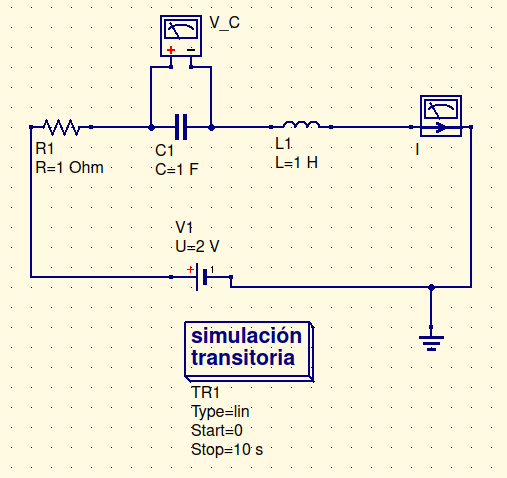
\includegraphics[scale=0.5]{circ.png}
\centering
\caption{Circuito de estudio.}
\label{fig:circ}
\end{figure}
Acá se agregan un medidor de tensión eléctrica entre los extremos del capacitor y un medidor de corriente electrica en la linea única del circuito, de manera que sea posible medir las variables anteriormente planteadas $V_C$ e $I$. Se realiza una simulación transitoria, lo que permite captar la evolución temporal de las variables de control ($I$ y $V_C$), para valores de tiempo entre $0 s$ y $10 s$. Los resultados de la simulación pueden apreciarse en la gráfica \ref{fig:ig} para la corriente $I$, y \ref{fig:vcg} para la tensión $V_C$


\begin{figure}[h]
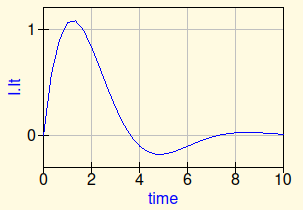
\includegraphics[scale=0.8]{ig.png}
\centering
\caption{Evolución temporal de la corriente $I$. Escala de corriente en Ampere y de tiempo en segundos.}
\label{fig:ig}
\end{figure} \newpage
\begin{figure}[h]
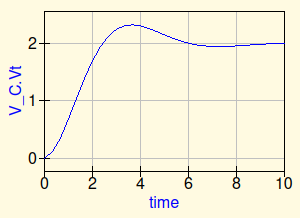
\includegraphics[scale=0.8]{vcg.png}
\centering
\caption{Evolución temporal de la tensión $V_C$. Escala de tensión en voltios y de tiempo en segundos.}
\label{fig:vcg}
\end{figure}

\subsubsection*{Análisis de resultados}

Tanto $V_C$ como $I$ presentan un comportamiento similar, oscilan de manera amortiguada en torno a un valor de equilibrio, estos serían $V_C=2v$ e $I=0$, lo que tiene mucho sentido cuando consideramos que este sería el comportamiento esperable en un régimen estacionario (o cuando $t \longrightarrow \infty$). Este comportamiento además concuerda con las soluciones náliticas obtenidas para el las variables $V_C$ \eqref{vc1} e $I$ \eqref{it1}.

\end{document}